\documentclass[../TDAM3.tex]{subfiles}%

\begin{document}
\section{Trioxyde de tungstène}
\enonce{%
	\begin{isd}
		Le trioxyde de tungstène \ce{WO3} solide est, en première approche, un solide
		ionique. Il présente une structure cubique telle que les ions tungstène
		\ce{W^{6+}} occupent les sommets de la maille et les ions oxyde \ce{O^{2-}} le
		milieu des arêtes. On note $a$ le paramètre de maille.
		\tcblower
		\begin{center}
			\captionof{table}{Données des rayons ioniques.}
			\label{tab:wo3}
			\begin{tabular}[c]{lcccccc}
				\toprule
				Espèce                 & \ce{H+}   & \ce{Li+}   & \ce{Na+}   & \ce{K+}   & \ce{O^{2-}} & \ce{W^{6+}}
				\\\midrule
				$r\ind{ion}$ (\si{pm}) & \num{e-5} & \num{78.0} & \num{98.0} & \num{133}
				                       & \num{132} & \num{62.0}
				\\\bottomrule
			\end{tabular}
		\end{center}
	\end{isd}
}%
\QR{%
	Dessiner une maille et vérifier la stœchiométrie du cristal.
}{%
	Voir figure. On a $8\times1/8 = 1$ cation \ce{W^{+6}}, et $12\times1/4 =
		3$ anions \ce{O^{2+}}, d'où la stœchiométrie.
	\begin{figure}[h]
		\centering
		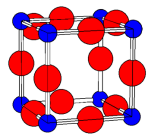
\includegraphics[scale=1]{tungstene}
		\caption{Maille élémentaire du trioxyde de tungstène. Les anions sont en
			rouge, les cations en bleu.}
		\label{fig:tung}
	\end{figure}
}%

\QR{%
	On admet une tangence cation-anion. Calculer la compacité du cristal
	\ce{WO3}.
}{%
	Contact anion-cation sur une arête, soit $a = r_{\ce{W}} + 2r_{\ce{O}} =
		\SI{338}{pm}$. D'où la compacité,
	\[
		\boxed{
			\frac{
				\frac{4}{3}\pi r_{\ce{W}}^{3} + 3\times \frac{4}{3}\pi
				r_{\ce{O}}^{3}}{
				(2r_{\ce{W}} + 2r_{\ce{O}})^{3}
			}
			= \num{0.51}
		}
	\]
}%

\QR{%
	Le centre du cube et les centres des faces de la maille dessinée
	précédemment sont vides. Calculer le rayon maximal d'un hétéroélément qui
	pourrait s'insérer dans ces sites sans déformation de la structure.
}{%
	Les anions \ce{O^{2-}} ont un rayon ionique supérieur aux cations
	\ce{W^{6+}}~: ce sont eux qui contraignent l'habitabilité. Pour loger un
	hétéroélement au centre d'une face, il faut que son rayon $r$ soit tel que
	\[
		2r_{\ce{O}} + 2r \leq a
		\qqsoit
		\boxed{r \leq \frac{a}{2} - r_{\ce{O}} = \SI{62}{pm}}
	\]
	Pour loger un hétéroélement au centre du cube, la contrainte est imposée par
	les anions au centre de deux arêtes opposées le long de la diagonale
	du cube (dans le plan à $z = a/2$). Ainsi,
	\[
		2r_{\ce{O}} + 2r \leq a \sqrt{2}
		\qqsoit
		\boxed{r \leq \frac{a \sqrt{2}}{2} - r_{\ce{O}} = \SI{142}{pm}}
	\]
}%

\QR{%
	On observe expérimentalement que les cations \ce{M^{+}}, avec \ce{M} qui
	peut être \ce{H}, \ce{Li}, \ce{Na} ou \ce{K}, peuvent s'insérer dans le
	cristal et occupent tous le même type de site. En déduire de quel site il
	s'agit.
}{%
	\ce{H+} pourrait s'insérer dans les deux types de sites, mais les autres
	cations alcalins ne peuvent s'insérer \textbf{qu'au centre du cube}.
}%

\end{document}
